\chapter{PHƯƠNG PHÁP NGHIÊN CỨU}

\section{Tiền Xử Lý Dữ Liệu và Làm Sạch}

Quá trình khám phá dữ liệu (EDA) trên 30.000 hồ sơ khách hàng cho thấy hai vấn đề lớn cần xử lý: sự mất cân bằng dữ liệu và hiện tượng đa cộng tuyến. 

Về phân phối nhãn, dữ liệu thể hiện sự mất cân bằng phân lớp (Class Imbalance) đáng kể: nhóm khách hàng có hành vi vỡ nợ (Default - nhãn 1) chỉ bao gồm 6.636 bản ghi (chiếm tỷ lệ 22.12\%), trong khi nhóm khách hàng thanh toán đúng hạn (Non-Default - nhãn 0) chiếm đa số tuyệt đối với 23.364 bản ghi (77.88\%).

\begin{figure}[H]
    \centering
    
\includegraphics[width=0.7\textwidth]{images/target_distribution_countplot.png}
    \caption{Phân bố biến mục tiêu cho thấy sự mất cân bằng trầm trọng của nhóm nợ xấu (Default)}
    \label{fig:target_dist}
\end{figure}

Bên cạnh đó, phân tích ma trận tương quan (Correlation Heatmap) bộc lộ hiện tượng đa cộng tuyến (Multicollinearity) rất mạnh giữa các biến dư nợ hóa đơn của các tháng liên tiếp (từ \texttt{BILL\_AMT1} đến \texttt{BILL\_AMT6}). Đặc điểm này là cơ sở quan trọng để nhóm tiến hành Kỹ nghệ đặc trưng (Feature Engineering) nhằm tổng hợp thông tin và loại bỏ các biến dư thừa ở giai đoạn sau.

\begin{figure}[H]
    \centering
    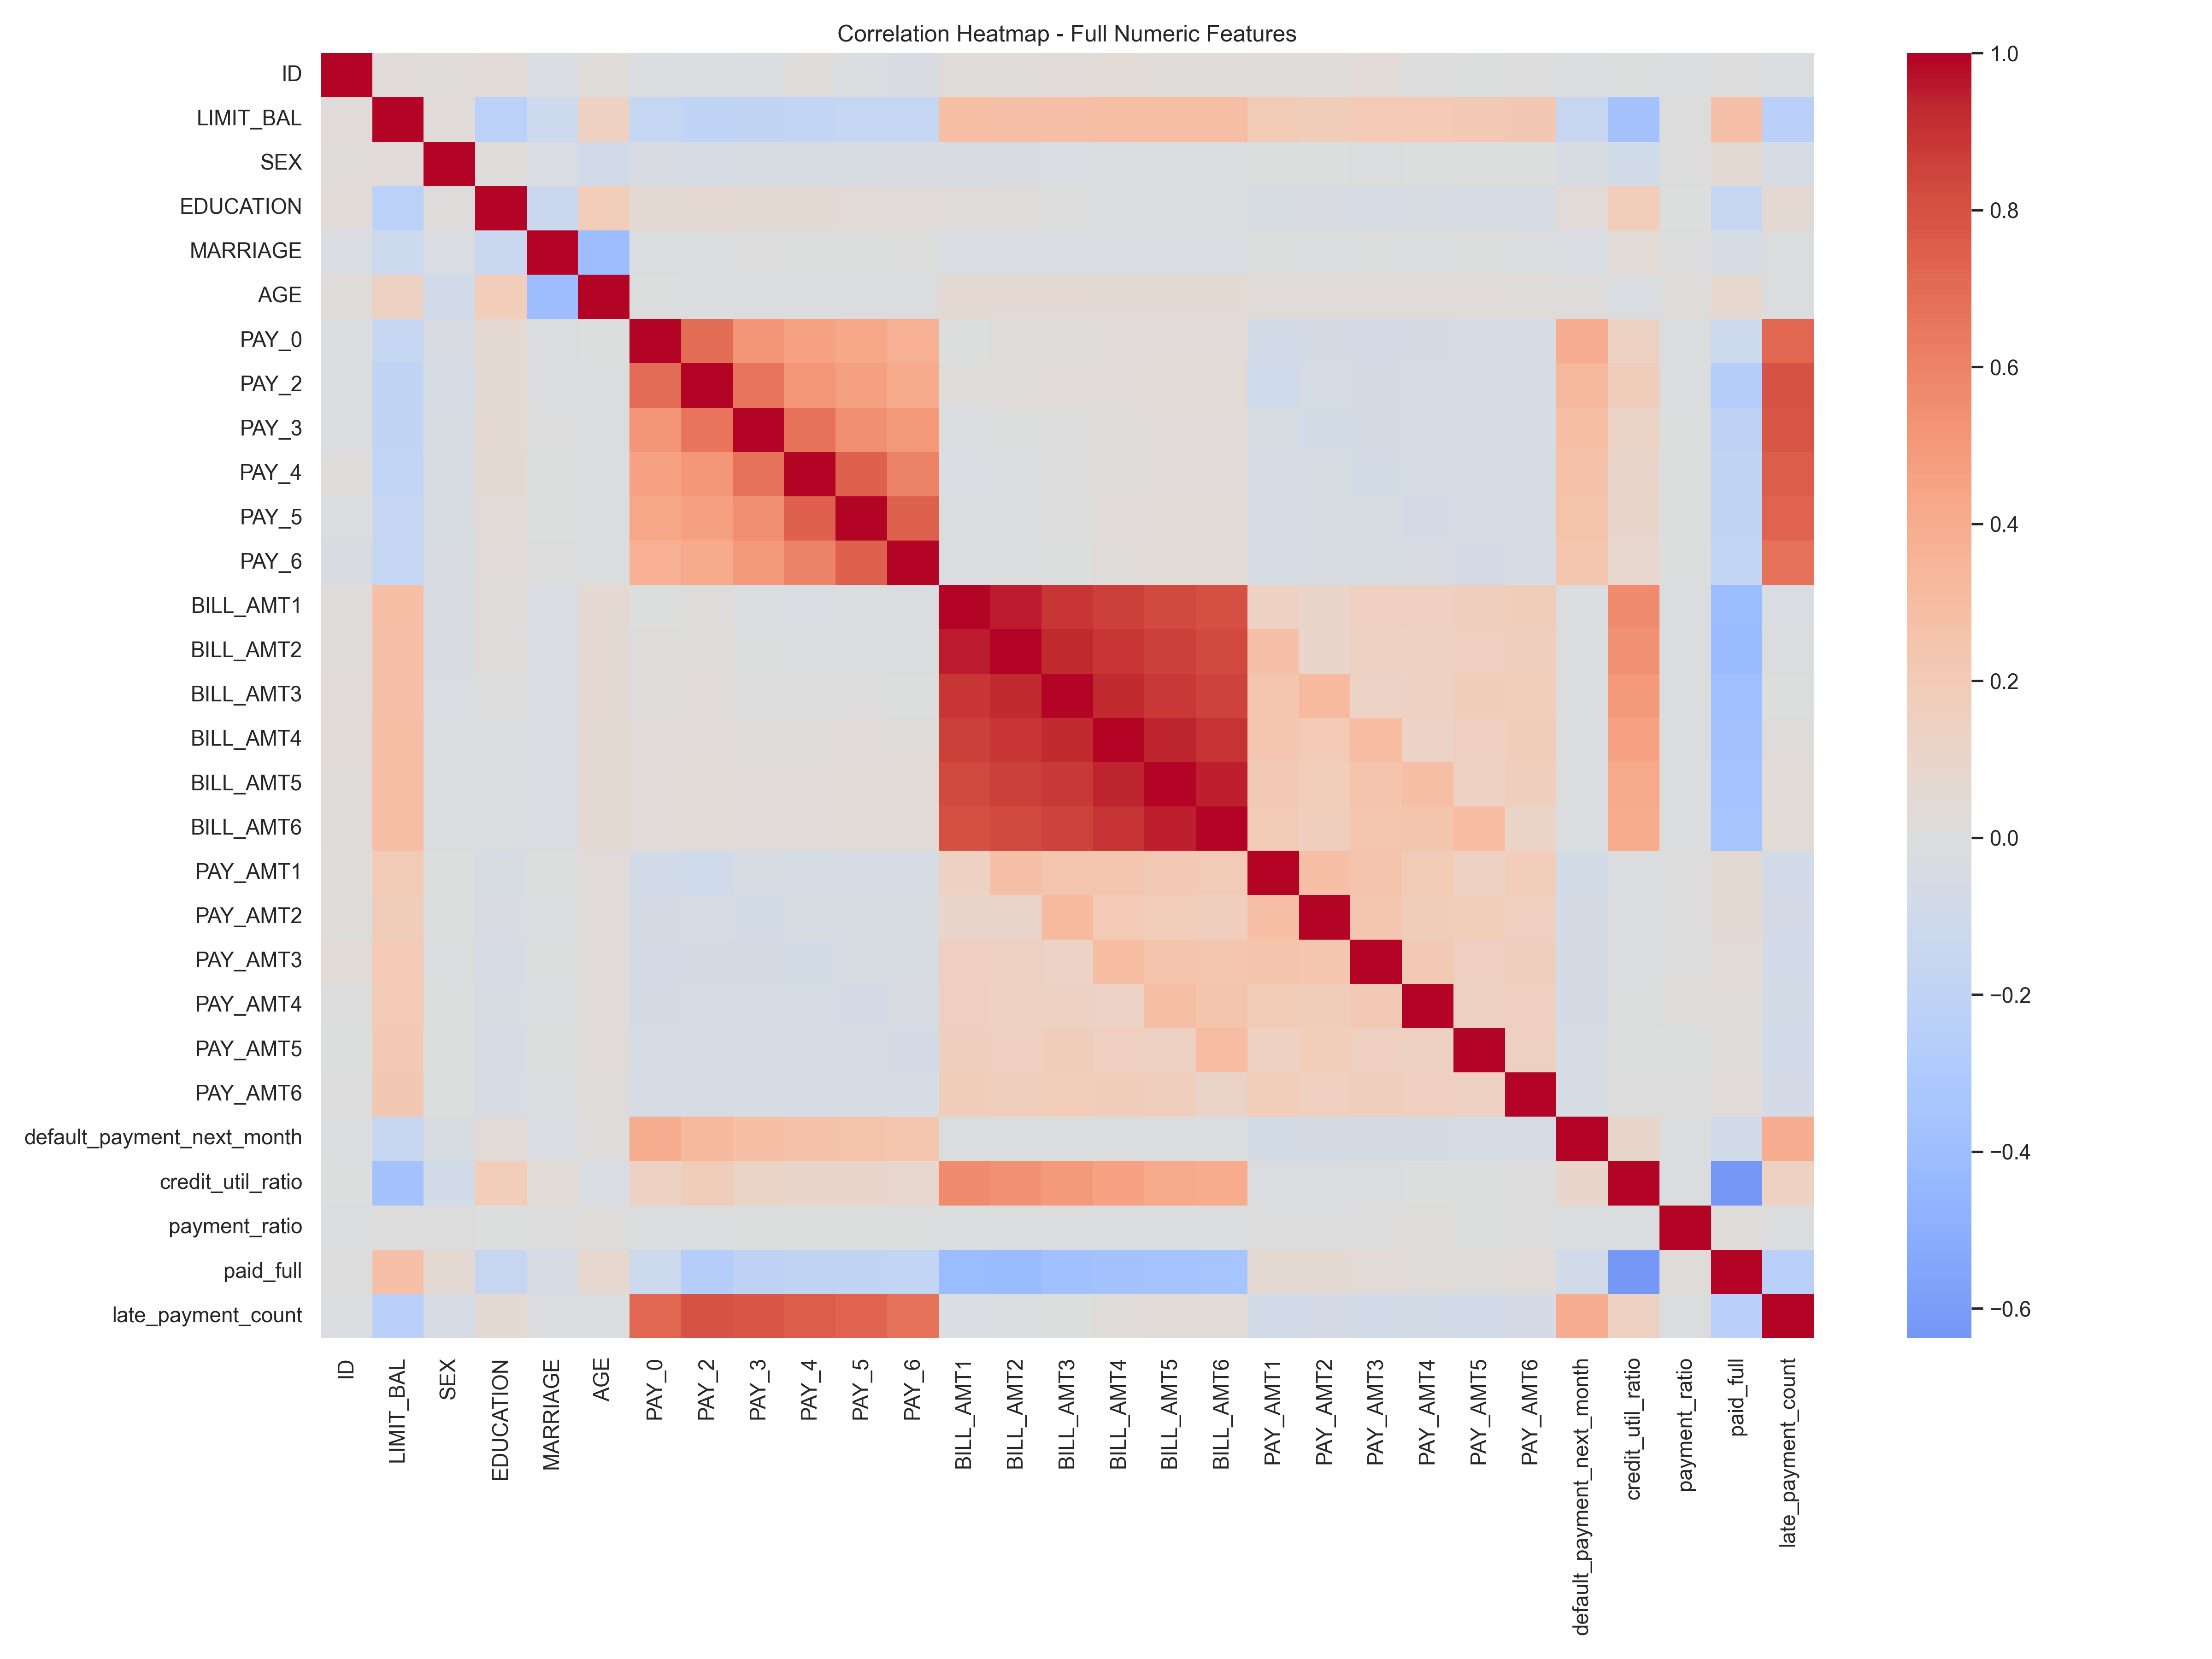
\includegraphics[width=0.8\textwidth]{images/correlation_heatmap_full.png}
    \caption{Ma trận tương quan (Correlation Heatmap) phản ánh hiện tượng đa cộng tuyến}
    \label{fig:correlation_heatmap}
\end{figure}

Dựa trên các phân tích trên, quy trình làm sạch dữ liệu (Data Cleaning) được thực hiện nghiêm ngặt theo các bước sau:

\subsection{Xử lý các biến phân loại (Categorical Features)}
\begin{itemize}
    \item \textbf{Biến \texttt{EDUCATION} (Trình độ học vấn):} Khảo sát phân phối cho thấy các giá trị nằm ngoài từ điển dữ liệu (0, 4, 5, 6) chiếm tỷ lệ rất nhỏ ($< 1\%$). Nghiên cứu đã gộp toàn bộ các giá trị này vào nhóm \textit{Other} (mã 4) nhằm giảm nhiễu, giúp thuật toán tập trung phân vùng các nhóm học vấn cốt lõi (Graduate School, University, High School).
    \item \textbf{Biến \texttt{MARRIAGE} (Tình trạng hôn nhân):} Tương tự, thuộc tính này chứa các giá trị 0 không được giải thích trong tài liệu gốc. Để đảm bảo tính nhất quán, các giá trị 0 được đồng bộ hóa vào nhóm \textit{Other} (mã 3), giữ nguyên tính toàn vẹn của hai nhóm khách hàng chính là Married và Single.
\end{itemize}

\subsection{Chuẩn hóa các biến trạng thái thanh toán (\texttt{PAY\_0} đến \texttt{PAY\_6})}
Trong bộ dữ liệu gốc, các giá trị -2 và -1 biểu thị khách hàng thanh toán dư hoặc trả hoàn toàn trước hạn; giá trị 0 biểu thị trạng thái thanh toán đúng hạn số tiền tối thiểu; trong khi các giá trị $\ge 1$ phản ánh số tháng nợ quá hạn. Nhằm chuẩn hóa các hành vi này thành một thang đo trễ hạn duy nhất, nghiên cứu áp dụng phép biến đổi cắt ngắn (clipping) tại ngưỡng 0:
\begin{equation}
    \text{PAY\_x\_clipped} = \max(0, \text{PAY\_x})
\end{equation}
Cụ thể, tất cả các lần trả nợ sớm hoặc trả đúng hạn đều được chuẩn hóa về cùng giá trị 0. Cách làm này giúp lược bỏ các nhiễu dữ liệu từ nhóm hành vi tín dụng an toàn, ép mô hình phải hội tụ trọng số và tập trung hoàn toàn vào việc nhận diện các dấu hiệu trễ hạn (late payment attributes).
\section{Kỹ Nghệ Đặc Trưng (Feature Engineering)}

Hiệu quả của các mô hình dự báo rủi ro tín dụng hiện đại phụ thuộc rất lớn vào khả năng định lượng các hành vi tín dụng cận biên của khách hàng. Dựa trên các trường dữ liệu gốc ($LIMIT\_BAL, BILL\_AMT, PAY\_AMT, PAY\_X$), nghiên cứu đã trích xuất ba nhóm đặc trưng phái sinh cốt lõi. Bước cải tiến này giúp chuyển đổi trọng tâm phân tích của mô hình từ việc chỉ sử dụng các giá trị tuyệt đối sang việc đánh giá dựa trên tần suất và xu hướng hành vi.

\subsection{Tỷ Lệ Sử Dụng Hạn Mức Tín Dụng (Credit Utilization Ratio)}
Đặc trưng này đo lường mức độ sử dụng tín dụng thực tế so với tổng hạn mức được ngân hàng cấp cho mỗi cá nhân. Công thức được xác định như sau:
\begin{equation}
    \text{credit\_util\_ratio} = \max\left(0, \frac{\text{BILL\_AMT1}}{\text{LIMIT\_BAL}}\right)
\end{equation}
Từ góc độ Quản trị rủi ro, khi tỷ lệ $\text{credit\_util\_ratio}$ tiến dần đến 1, nó phản ánh khách hàng đang cạn kiệt thanh khoản tiền mặt và phụ thuộc hoàn toàn vào thẻ tín dụng. Đây là một tín hiệu cảnh báo quan trọng và là biến dự báo có mức độ tương quan cao với xác suất vỡ nợ (Default) của khách hàng.

\subsection{Tỷ Lệ Thanh Toán (Payment Ratio)}
Đặc trưng này đo lường tỷ lệ số tiền khách hàng đã thực trả so với dư nợ hóa đơn của kỳ trước đó:
\begin{equation}
    \text{payment\_ratio} = \max\left(0, \frac{\text{PAY\_AMT1}}{\text{BILL\_AMT2}}\right)
\end{equation}
Về mặt lập trình, để xử lý các ngoại lệ toán học khi $\text{BILL\_AMT2} = 0$ (gây ra lỗi Division by Zero dẫn đến giá trị Infinity hoặc NaN), thuật toán được thiết lập để mặc định gán tỷ lệ này bằng 0. Bên cạnh đó, nghiên cứu trích xuất thêm biến cờ nhị phân (binary feature) \textit{paid\_full}. Biến này nhận giá trị $1$ khi $\text{PAY\_AMT1} \geq \text{BILL\_AMT2}$, đánh dấu việc khách hàng đã hoàn thành toàn bộ nghĩa vụ thanh toán cho dư nợ kỳ trước.

\subsection{Tần Suất Chậm Thanh Toán (Late Payment Count)}
Đặc trưng này tổng hợp số lần khách hàng bị ghi nhận trễ hạn trong suốt chu kỳ 6 tháng quan sát (dựa trên các trường trạng thái $\text{PAY\_0}$ và $\text{PAY\_2}$ đến $\text{PAY\_6}$):
\begin{equation}
    \text{late\_payment\_count} = \sum_{i \in \{0, 2, 3, 4, 5, 6\}} \mathbb{I}(\text{PAY\_i} > 0)
\end{equation}
Việc các trạng thái thanh toán mang giá trị $>0$ (tương ứng với chậm trả nợ từ 1 tháng trở lên) phản ánh sự bất ổn trong hành vi tài chính của khách hàng. Thực nghiệm cho thấy, tần suất vi phạm này là một chỉ báo rủi ro cực kỳ mạnh, liên tục giữ vị trí dẫn đầu về độ quan trọng trong các mô hình cây quyết định.

\section{Xử lý Mất Cân Bằng Dữ Liệu - Kỹ Thuật SMOTE}

Trong tập dữ liệu thực tế, nhóm khách hàng vỡ nợ (Default) chỉ chiếm tỷ lệ 22.12\%, tạo ra bài toán mất cân bằng dữ liệu. Việc đưa trực tiếp tập dữ liệu gốc vào huấn luyện sẽ khiến các thuật toán học máy gặp hiện tượng thiên kiến lớp đa số (Majority Class Bias), dẫn đến mô hình có xu hướng dự đoán toàn bộ khách hàng đều trả nợ tốt để tối ưu hóa độ chính xác tổng thể (Accuracy).
Để khắc phục, nghiên cứu áp dụng kỹ thuật \textbf{SMOTE} (Synthetic Minority Over-sampling Technique). Thay vì nhân bản dữ liệu một cách đơn giản, SMOTE tạo ra các mẫu dữ liệu nhân tạo mới cho nhóm thiểu số dựa trên thuật toán k-láng giềng gần nhất (với $k=5$). Công thức nội suy sinh mẫu mới được thực hiện như sau:
\begin{equation}
    \mathbf{x}_{new} = \mathbf{x}_i + \lambda \times (\mathbf{x}_{neighbor} - \mathbf{x}_i)
\end{equation}
Trong đó, $\lambda$ là một số ngẫu nhiên trong khoảng $[0, 1]$ và $\mathbf{x}_{neighbor}$ là một trong 5 láng giềng gần nhất của mẫu $\mathbf{x}_i$.

\textbf{Phòng Ngừa Rò Rỉ Dữ Liệu (Data Leakage Prevention):} Để đảm bảo tính khách quan cho mô hình, bộ dữ liệu 30.000 mẫu ban đầu được chia thành hai tập: \textbf{Tập Huấn luyện} (Train Set - 80\%) và \textbf{Tập Kiểm thử} (Test Set - 20\%) có sử dụng tham số phân tầng ($\text{stratify} = \mathbf{y}$) để giữ nguyên tỷ lệ mất cân bằng ban đầu ở cả hai tập. Tập Huấn luyện chứa 24.000 mẫu, bao gồm 18.691 mẫu nhãn 0 và 5.309 mẫu nhãn 1.

Một nguyên tắc cực kỳ nghiêm ngặt được áp dụng là: Kỹ thuật SMOTE \textbf{chỉ được thực hiện duy nhất trên Tập Huấn luyện}. Sau khi áp dụng, SMOTE đã sinh thêm 13.382 mẫu nhân tạo cho nhóm vỡ nợ, cân bằng tỷ lệ nhãn 0 và 1 đạt mức 50:50. Kích thước Tập Huấn luyện lúc này tăng lên 37.382 mẫu.

Tập Kiểm thử (gồm 6.000 mẫu) hoàn toàn không chịu sự can thiệp của SMOTE. Việc giữ nguyên vẹn tập Kiểm thử giúp đánh giá chính xác khả năng tổng quát hóa của mô hình trên dữ liệu thực tế chưa từng thấy, ngăn chặn hoàn toàn rủi ro rò rỉ dữ liệu và đánh giá quá mức hiệu năng thực sự (Over-fitting).

\section{Quy trình chuyển đổi dữ liệu và Chiến lược mô hình hóa (Modeling Strategy)}

\subsection{Đường ống chuyển đổi dữ liệu (Data Transformation Pipeline)}
Để đảm bảo các thuật toán học máy hoạt động ổn định và hội tụ nhanh, toàn bộ quá trình tiền xử lý dữ liệu trên tập Huấn luyện được đóng gói thông qua công cụ \textit{ColumnTransformer}. Dữ liệu được áp dụng các phương pháp chuyển đổi chuyên biệt tùy thuộc vào đặc tính của từng biến:
\begin{itemize}
    \item \textbf{Chuẩn hóa biến số thực (Numerical Scaling):} Các biến tài chính (\textit{LIMIT\_BAL, BILL\_AMT, PAY\_AMT}) thường có biên độ dao động giá trị rất lớn. Chúng tôi sử dụng \textit{StandardScaler} để chuẩn hóa các biến này theo phân phối chuẩn (Z-score normalization), đưa giá trị trung bình ($\mu$) về 0 và độ lệch chuẩn ($\sigma$) về 1:
    \begin{equation}
        z = \frac{x - \mu}{\sigma}
    \end{equation}
    Việc đưa dữ liệu về cùng một thang đo giúp các thuật toán dựa trên nền tảng hạ gradient (Gradient Descent) tối ưu hóa hàm mất mát trơn tru hơn, tránh tình trạng trọng số bị cập nhật lệch hướng do chênh lệch tỷ lệ (scale).
    
    \item \textbf{Mã hóa biến phân loại (One-Hot Encoding):} Các biến định danh (\textit{SEX, EDUCATION, MARRIAGE}) được chuyển đổi sang dạng vector nhị phân thông qua \textit{OneHotEncoder}. Phương pháp này triệt tiêu hoàn toàn rủi ro mô hình hiểu nhầm các con số định danh thành các giá trị có tính thứ bậc (ordinal relationship). Ví dụ, việc mã hóa giúp thuật toán không đánh giá tình trạng hôn nhân loại "2" có trọng số hoặc ý nghĩa gấp đôi loại "1".
\end{itemize}

\subsection{Mô hình cơ sở (Baseline Model)}
Nghiên cứu lựa chọn mô hình \textbf{Hồi quy Logistic} (Logistic Regression) làm mô hình cơ sở (Baseline Model). Dựa trên hàm Sigmoid, mô hình tính toán xác suất vỡ nợ của khách hàng thông qua phương trình:
\begin{equation}
    P(Y=1|X) = \frac{1}{1 + e^{-(\beta_0 + \beta_1 X_1 + \cdots + \beta_n X_n)}}
\end{equation}
Điểm ROC-AUC sinh ra từ mô hình phân loại tuyến tính này đóng vai trò là ngưỡng hiệu năng chuẩn (benchmark). Các mô hình học tập tổng hợp (Ensemble Learning) phức tạp được áp dụng sau đó bắt buộc phải chứng minh được sự vượt trội rõ rệt so với ngưỡng điểm này để bù đắp cho chi phí tài nguyên tính toán gia tăng.

\subsection{Nhóm mô hình học dựa trên cây (Tree-Based Models)}
Để xử lý hiệu quả các mối quan hệ phi tuyến tính phức tạp và tận dụng tối đa sức mạnh của các đặc trưng do nhóm tạo ra (như $late\_payment\_count$), nghiên cứu triển khai hai thuật toán Gradient Boosting tiên tiến nhất hiện nay:
\begin{itemize}
    \item \textbf{XGBoost (Extreme Gradient Boosting):} Thuật toán này tích hợp sẵn cơ chế điều chuẩn (L1/L2 Regularization) giúp kiểm soát chặt chẽ hiện tượng quá khớp (Overfitting). XGBoost phát triển các nhánh cây theo từng mức (Level-wise Growth), ưu tiên tính ổn định cao trong quá trình phân tách các nút quyết định.
    \item \textbf{LightGBM:} Vượt trội về tốc độ xử lý trên tập dữ liệu lớn nhờ cơ chế phát triển cây theo lá (Leaf-wise Growth). Thuật toán này ưu tiên mở rộng các lá có độ giảm suy hao lớn nhất thay vì mở rộng đồng đều. Dù mang lại độ chính xác cao hơn, cơ chế này nhạy cảm hơn với hiện tượng quá khớp, do đó yêu cầu sự kiểm soát nghiêm ngặt đối với siêu tham số độ sâu tối đa (\text{max\_depth}).
\end{itemize}

\subsection{Tối ưu hóa siêu tham số với Optuna (Hyperparameter Tuning)}
Các thuật toán như XGBoost và LightGBM chỉ phát huy tối đa sức mạnh khi bộ siêu tham số (Hyperparameters) được tinh chỉnh hợp lý. Thay vì sử dụng phương pháp tìm kiếm theo lưới (Grid Search) truyền thống vốn cạn kiệt tài nguyên tính toán, nghiên cứu ứng dụng thư viện \textbf{Optuna}.

Optuna sử dụng thuật toán Tối ưu hóa Bayes, cụ thể là mô hình TPE (Tree-structured Parzen Estimator). Thuật toán này phân tích các vòng chạy (trials) trong quá khứ để xác định vùng không gian tham số tiềm năng nhất, từ đó hướng tới việc cực đại hóa điểm số $ROC\_AUC$. Các tham số cốt lõi được đưa vào không gian tìm kiếm bao gồm:
\begin{itemize}
    \item \textbf{learning\_rate ($\eta$):} Điều chỉnh tốc độ học (bước nhảy) của mô hình, giúp tìm điểm cân bằng giữa tốc độ hội tụ và độ chính xác.
    \item \textbf{max\_depth \& num\_leaves:} Quản lý độ phức tạp cấu trúc cây, đóng vai trò là rào chắn quan trọng nhất để ngăn chặn tình trạng mô hình học vẹt (Overfitting) từ dữ liệu huấn luyện gốc.
    \item \textbf{subsample \& colsample\_bytree:} Tỷ lệ lấy mẫu con ngẫu nhiên đối với các hàng (data points) và cột (features). Cơ chế ngẫu nhiên hóa này giúp giảm phương sai (variance) của mô hình và ngăn thuật toán bị kẹt tại các điểm cực tiểu địa phương (Local Minima).
\end{itemize}

\section{Đánh giá Hiệu năng và Khả năng Giải thích của Mô hình (Metrics \& Explainable AI)}

\subsection{Các độ đo đánh giá hiệu năng (Performance Metrics)}
Hệ thống đánh giá rủi ro tín dụng được đo lường thông qua các chỉ số chuyên dụng, phù hợp với đặc thù của dữ liệu tài chính:
\begin{itemize}
    \item \textbf{ROC-AUC:} Đánh giá khả năng phân tách giữa hai lớp (Vỡ nợ và Không vỡ nợ) của mô hình. Đây là thước đo đáng tin cậy và không bị phụ thuộc vào tỷ lệ phân bố của dữ liệu, đặc biệt phù hợp cho bài toán mất cân bằng lớp (Imbalanced Data).
    \item \textbf{Recall (Độ nhạy - Sensitivity):} Tỷ lệ khách hàng thực sự vỡ nợ được mô hình nhận diện đúng ($\frac{TP}{TP + FN}$). Trong lĩnh vực tín dụng, việc dự báo sót một khách hàng có rủi ro vỡ nợ (False Negative) sẽ gây ra thiệt hại tài chính nặng nề. Do đó, Recall là chỉ số được ưu tiên hàng đầu khi tinh chỉnh và lựa chọn mô hình.
    \item \textbf{Precision \& F1-Score:} Precision giúp đo lường tỷ lệ dự báo chính xác trên tổng số cảnh báo vỡ nợ, từ đó kiểm soát số lượng cảnh báo giả (False Positive). F1-Score là trung bình điều hòa giữa Recall và Precision, giúp đánh giá sự cân bằng tổng thể của mô hình khi có sự đánh đổi (trade-off) giữa hai chỉ số này.
\end{itemize}

\begin{figure}[H]
    \centering
    
\includegraphics[width=0.8\textwidth]{images/final_roc_comparison.png}
    \caption{Đường cong ROC và diện tích dưới đường cong (AUC) của các mô hình phân loại}
    \label{fig:roc_curve}
\end{figure}

\begin{figure}[H]
    \centering
    
\includegraphics[width=0.6\textwidth]{images/confusion_xgb_tuned.png}
    \caption{Ma trận nhầm lẫn (Confusion Matrix) của mô hình XGBoost sau khi tối ưu siêu tham số}
    \label{fig:confusion_matrix}
\end{figure}

\subsection{Khả năng giải thích mô hình với SHAP (Explainable AI - XAI)}
Các thuật toán học máy mạnh mẽ (như Gradient Boosting) thường bị xem là các "Hộp đen" (Black Box) do cấu trúc cây quyết định phi tuyến tính phức tạp, gây khó khăn cho việc giải thích lý do đằng sau mỗi quyết định cấp tín dụng. Để giải quyết rào cản này, nghiên cứu áp dụng kỹ thuật \textbf{Explainable AI (XAI)} thông qua thư viện \textit{SHAP (SHapley Additive exPlanations)}. 

Cụ thể, thuật toán \texttt{TreeExplainer} được sử dụng để tính toán giá trị Shapley ($\phi_i$), nhằm định lượng mức độ đóng góp của từng đặc trưng vào kết quả dự đoán xác suất vỡ nợ cuối cùng:
\begin{equation}
    f(x) = g_0 + \sum_{i=1}^{M} \phi_i
\end{equation}

\begin{figure}[H]
    \centering
    
\includegraphics[width=0.9\textwidth]{images/feature_importance_best.png}
    \caption{Mức độ quan trọng của Top 10 đặc trưng đối với kết quả dự báo của mô hình (Feature Importance)}
    \label{fig:feature_importance}
\end{figure}

\begin{figure}[H]
    \centering
    
\includegraphics[width=0.8\textwidth]{images/shap_summary_lgb_best.png}
    \caption{Biểu đồ SHAP Summary Plot thể hiện chiều tác động của các đặc trưng đến xác suất vỡ nợ}
    \label{fig:shap_summary}
\end{figure}

Công cụ SHAP cung cấp hai góc nhìn minh bạch và sâu sắc cho mô hình. Thứ nhất, nó xác định rõ các đặc trưng mang tính quyết định (Top Features) như tần suất chậm thanh toán (\textit{late\_payment\_count}), trạng thái tháng gần nhất (\textit{PAY\_0}), và hạn mức tín dụng (\textit{LIMIT\_BAL}). Thứ hai, thông qua biểu đồ Summary Plot (Hình \ref{fig:shap_summary}), SHAP hiển thị rõ \textbf{chiều tác động (Directional Impact)} của từng đặc trưng lên xác suất vỡ nợ.

Dựa trên biểu đồ SHAP Summary Plot, ta có thể quan sát một quy luật thực tiễn: Các điểm dữ liệu có giá trị \textit{late\_payment\_count} cao (thể hiện bằng màu đỏ) luôn đi kèm với giá trị SHAP dương (nằm bên phải trục tung). Điều này chứng minh rằng, khi tần suất trễ hạn của khách hàng càng tăng, thuật toán sẽ đẩy mạnh xác suất dự báo khách hàng đó vào nhóm Vỡ nợ (Default). Tính minh bạch này không chỉ giúp kiểm chứng logic toán học của mô hình mà còn đáp ứng các tiêu chuẩn khắt khe về kiểm toán mô hình (Model Auditability), tạo cơ sở vững chắc để các chuyên gia tín dụng tin tưởng và ứng dụng vào thực tế.
